\documentclass{ctexbeamer}

% 使用 <thubeamer> 主题
% 模板选项如下
% (a.1) smoothbars: 页面顶端单行显示目录,默认选项
\usetheme[sectiontoc]{thubeamer}

\usepackage{media9}
\usepackage{listings}
\lstnewenvironment{textcode}{
  \lstset{
    basicstyle=\footnotesize\ttfamily,
    breaklines=true,
    frame=single,
    numbersep=2pt,
    xleftmargin=0.5em,
    framesep=1mm
  }
}{}


% (a.2) sidebar: 页面左侧分栏显示目录
% \usetheme[sidebar]{thubeamer}

% (b) sectiontoc: 在每节(section)前显示目录,并高亮显示当前节,默认不显示

% (c) subsectiontoc: 在每小节(subsection)前显示目录,并高亮显示当前节和当前小节,默认不显示

% (d) en: 仅使用英文来制作 beamer,应用此选项后,汉字将全部无法编译

% 图片存放路径

\graphicspath{{figures/}}

\include{macros}

% 封面信息,方括号内容是显示在左侧边栏的内容(当选择 sidebar 主题时有效)
\title[篮球高光检测]{篮球高光检测项目\\[2mm] 汇报}
\author[唐梓楠]{牛衍昌\\鲁继元\\唐梓楠\\[5mm] 导师:黄必清教授}
\institute[清华大学]{\small 清华大学}
\date{\small \vskip -10pt \today}

% 开始写文章
\begin{document}

% 标题页
\begin{frame}
  \maketitle
\end{frame}

% 目录页
\section*{目录}
\frame{
  \frametitle{\secname}
  \tableofcontents[hideallsubsections]
}

\section{Yolo12x 训练}

\begin{frame}{SportsMOT 数据集}

  \begin{block}{ICCV 2023}
    \textbf{SportsMOT: A Large Multi-Object Tracking Dataset in Multiple Sports Scenes}~\cite{Cui_2023_ICCV}
  \end{block}

  专业比赛运动场景的多目标追踪数据集,包括\textbf{篮球、排球、足球}。

  包含 \textbf{240 个三个类别的片段},均从 \textbf{YouTube} 上的\textbf{奥运会、NCAA 和 NBA} 中收集。仅下载\textbf{分辨率 720P}、\textbf{帧率 25 FPS} 且为\textbf{官方录制}的搜索结果。所有视频被手动剪辑为\textbf{平均 485 帧}的片段,片段内无镜头切换。

  足球比赛提供户外场景,其余为室内场景。比赛场地的视角各不相同,如 NBA 观众密集的侧面视角、排球发球区视角、足球空中俯视视角等。
\end{frame}

\begin{frame}{SportsMOT 数据集 Statstics}
  \begin{table}[h]
    \centering
    \resizebox{\linewidth}{!}{
    \begin{tabular}{lccccc}
      \toprule
      Category (avg.) & \#frames & \#tracks & track gap len & track length & \#bboxes per frame \\
      \midrule
      篮球 & 845.4 & 10 & 68.7 & 767.9 & 9.1 \\
      排球 & 360.4 & 12 & 38.2 & 335.9 & 11.2 \\
      足球 & 673.9 & 20.5 & 116.1 & 422.1 & 12.8 \\
      \bottomrule
    \end{tabular}
    }
  \end{table}

  \begin{columns}
    \begin{column}{0.5\textwidth}
      \begin{figure}[t]
        \centering
        \includegraphics[width=0.8\linewidth]{speed.png}
        \caption{速度分布(高斯概率密度函数)}
      \end{figure}
    \end{column}
    \begin{column}{0.5\textwidth}
      \begin{itemize}
        \item \textbf{track}: 每个视频的轨迹数量
        \item \textbf{tracklen}: 每个视频的平均长度/帧数
        \item \textbf{speed}: 视频中运动员的平均速度
      \end{itemize}
    \end{column}
  \end{columns}
\end{frame}

\begin{frame}{SportsMOT 数据集 Cases}
  \begin{columns}
    \begin{column}{0.33\textwidth}
      \begin{figure}[htbp]
        \centering
        \centering
        \includegraphics[width=\linewidth]{Basketball.png}
        \begin{center} \scriptsize 篮球(NBA) \end{center}
      \end{figure}
    \end{column}
    \begin{column}{0.33\textwidth}
      \begin{figure}[htbp]
        \centering
        \includegraphics[width=\linewidth]{Volleyball.png}
        \begin{center} \scriptsize 排球(2012 伦敦奥运会) \end{center}
      \end{figure}
    \end{column}
    \begin{column}{0.33\textwidth}
      \begin{figure}[htbp]
        \centering
        \includegraphics[width=\linewidth]{Football.png}
        \begin{center} \scriptsize 足球(英格兰足总杯) \end{center}
      \end{figure}
    \end{column}
  \end{columns}
\end{frame}

\begin{frame}{Yolo12x 训练情况}
  \begin{columns}
    \begin{column}{0.5\textwidth}
      \begin{figure}
        \centering
        \includegraphics[width=\linewidth]{yolo_train_result/results.png}
        \caption{训练 Loss 曲线}
      \end{figure}
    \end{column}
    \begin{column}{0.5\textwidth}
      \begin{figure}
        \centering
        \includegraphics[width=\linewidth]{yolo_train_result/val_batch0_labels.jpg}
        \includegraphics[width=\linewidth]{yolo_train_result/val_batch0_pred.jpg}
        \caption{验证集对比}
      \end{figure}
    \end{column}
  \end{columns}
\end{frame}

\begin{frame}{Yolo12x 训练后测试情况}
  \begin{columns}
    \begin{column}{0.5\textwidth}
      \begin{itemize}
        \item 先在整个数据集上训练
        \item 考虑到足球、排球与篮球场景差异较大,后尝试单独在篮球上训练
        \item 效果都变差
      \end{itemize}
      \textbf{可能的原因}:
      \begin{itemize}
        \item Yolo12x 本身足够强
        \item SportsMOT 为 720p 25fps,测试数据为 1080p 30fps
        \item SportsMOT 为专业球场,测试数据为野球场
      \end{itemize}
    \end{column}
    \begin{column}{0.5\textwidth}
      \begin{figure}
        \centering
        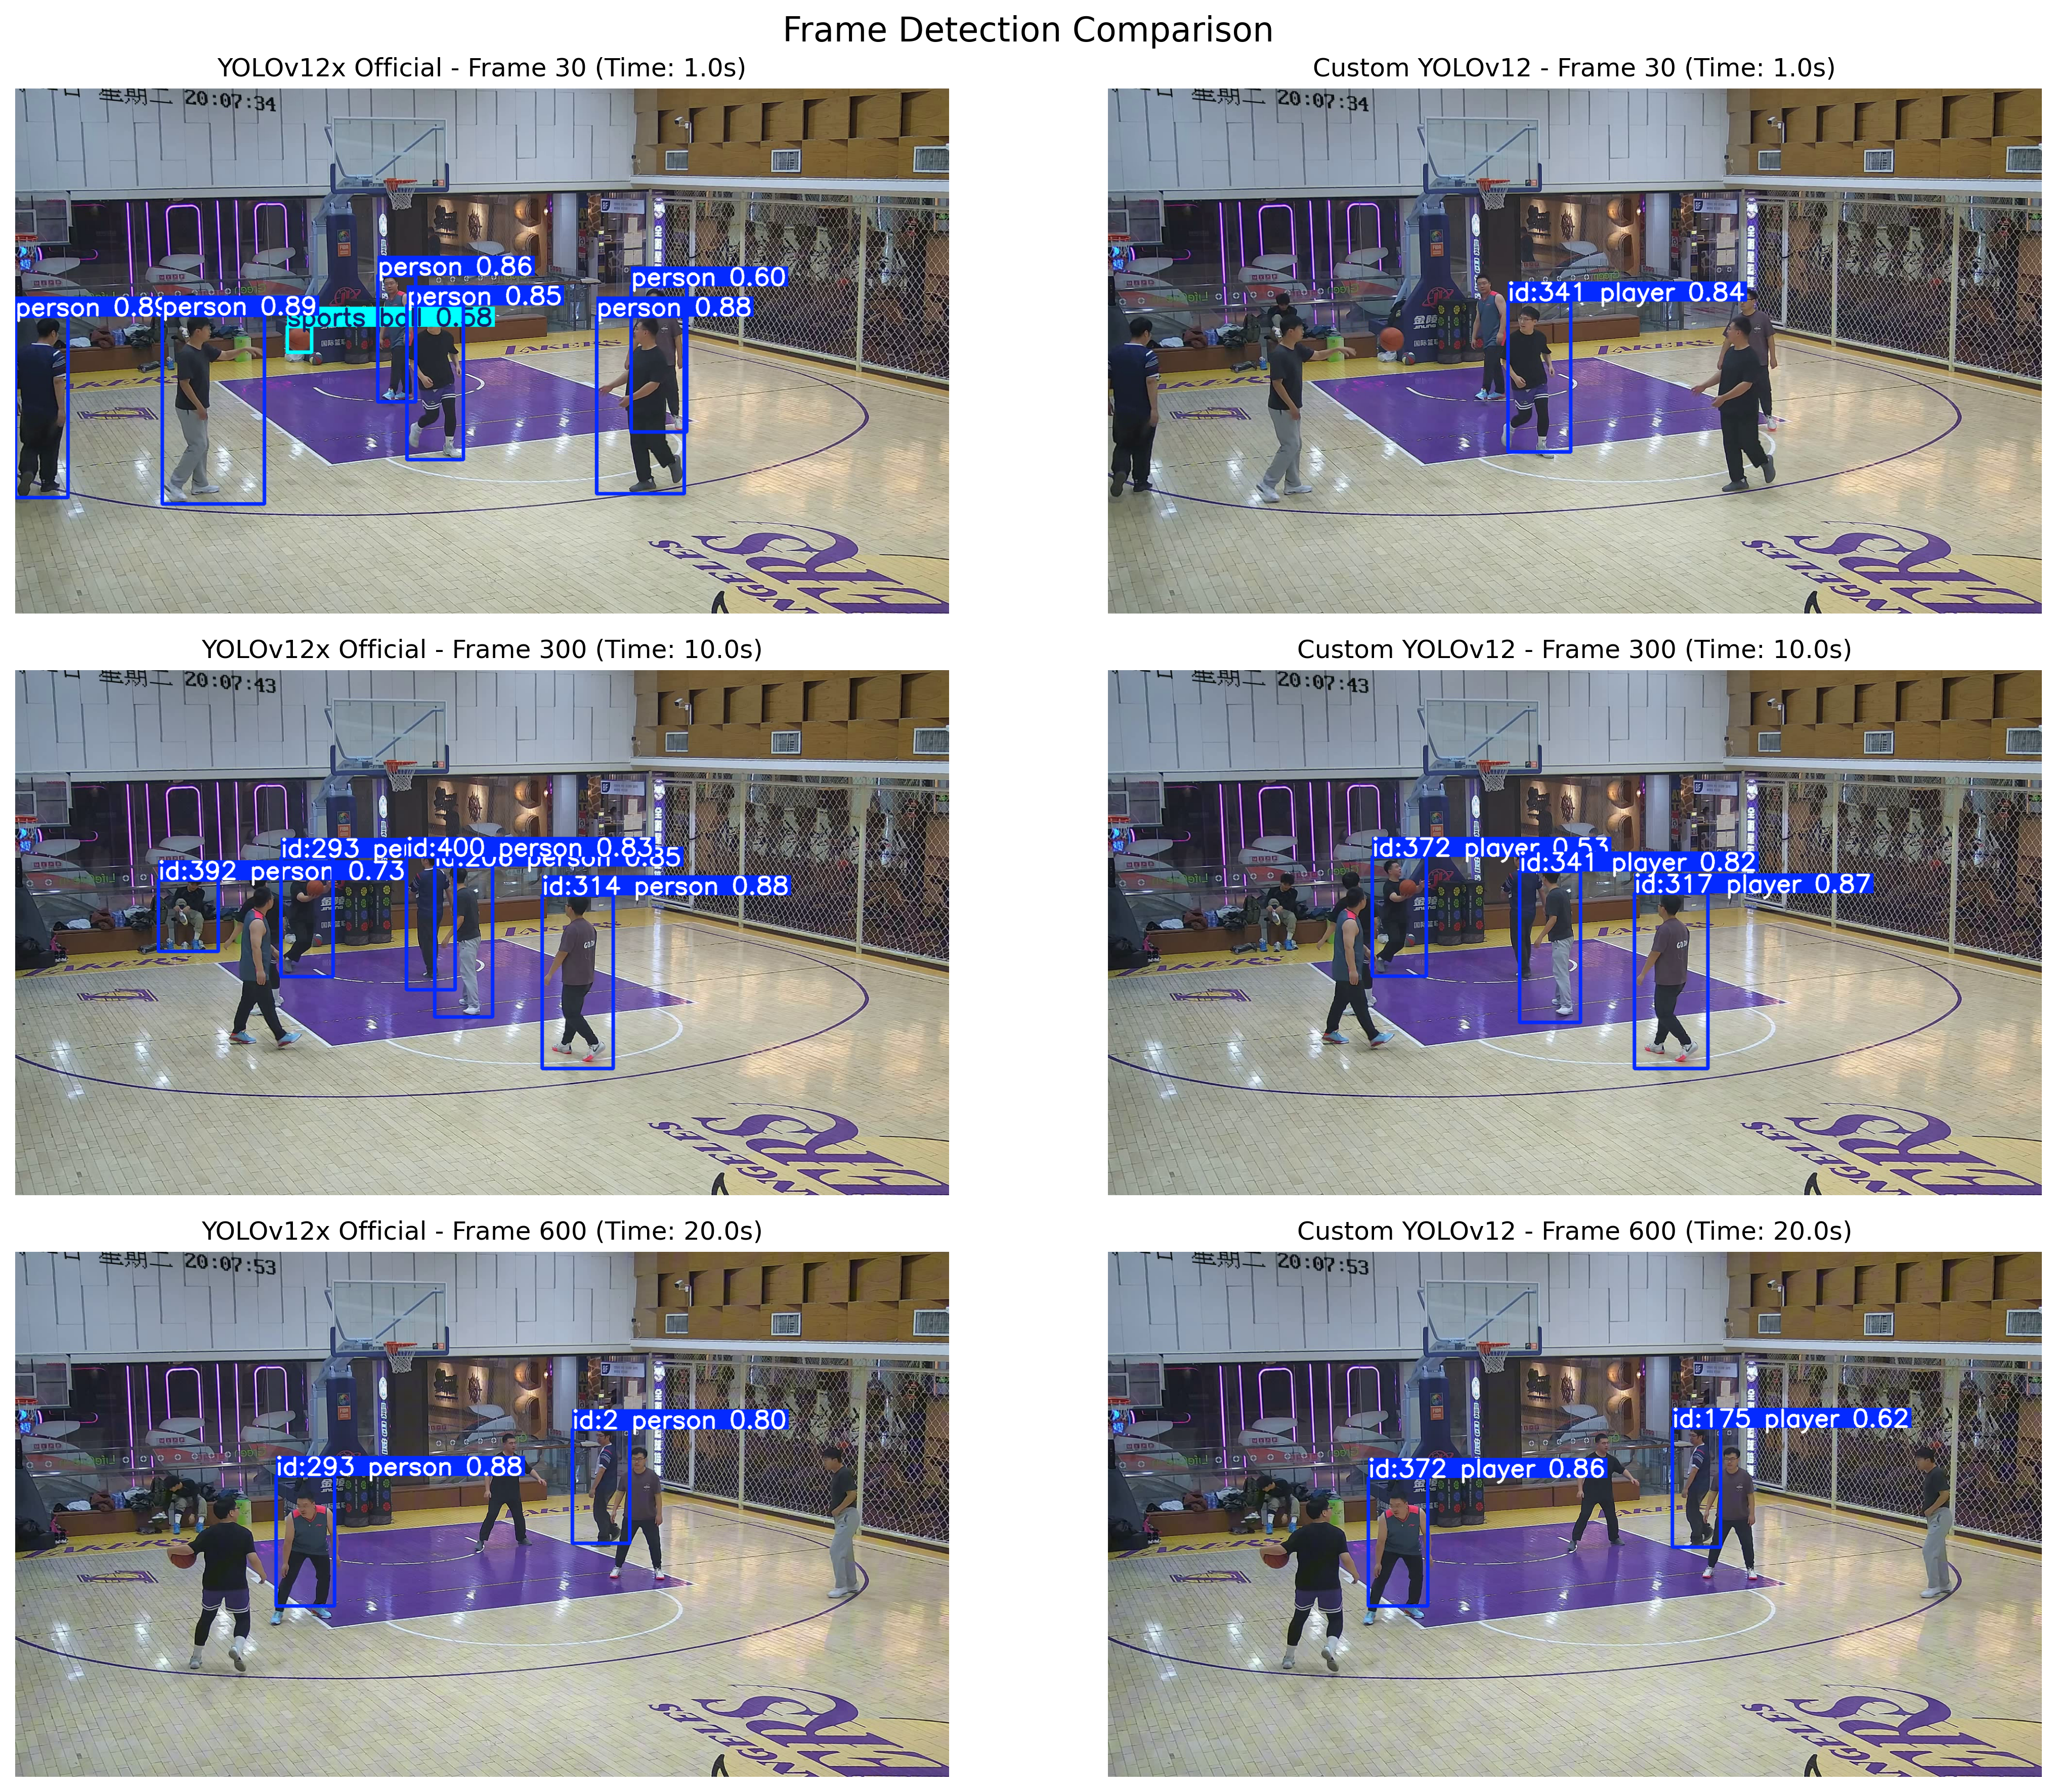
\includegraphics[width=\linewidth]{yolo_train_result/frame_comparison.png}
        \caption{Yolo12x 训练前后对比}
      \end{figure}
    \end{column}
  \end{columns}
\end{frame}

\begin{frame}{Yolo12x 训练后测试情况}
  \begin{figure}
    \centering
    \includegraphics[width=\linewidth]{yolo_train_result/confidence_trend.png}
  \end{figure}
\end{frame}

\section{畸变校正}

\begin{frame}[fragile]{A1 A2 相机内外参}
  \begin{block}{A1 内参}
    \begin{textcode}
# 相机内参矩阵格式: [[fx, 0, cx], [0, fy, cy], [0, 0, 1]]
camera_matrix = 
[[4144.1, 0, 1656.5],
[0, 4165.2, 918.5415],
[0, 0, 1]]

# 畸变系数
# 格式: [k1, k2, p1, p2, k3] (径向畸变+切向畸变)
dist_coeffs = [-1.3696, 4.0575, 0, 0, -6.7578]
    \end{textcode}
  \end{block}
\end{frame}

\begin{frame}[fragile]{A1 A2 相机内外参}
  \begin{block}{外参矩阵}
    \begin{textcode}
#A2 为主相机
#平移矩阵
[20514, 3244.5, 14648]

#旋转矩阵
[[0.4853, -0.3123, -0.8166]
[0.0900,  0.9469, -0.3087]
[0.8697, 0.0763, 0.4877]]

#外参矩阵
[[0.4853, -0.3123, -0.8166, 20514]
[0.0900,  0.9469, -0.3087, 3244.5]
[0.8697, 0.0763, 0.4877,14648]
[0, 0, 0,1]]
    \end{textcode}
  \end{block}
\end{frame}

\begin{frame}{去畸变前后效果对比}
  对于人脸识别与人员追踪有一定效果
  \begin{figure}
    \centering
    \includegraphics[width=\linewidth]{矫正对比/face_similarity_comparison_plot.png}
    \caption{人脸识别前后对比}
  \end{figure}
\end{frame}

\begin{frame}{去畸变前后效果对比}
  \begin{figure}
    \centering
    \includegraphics[width=\linewidth]{矫正对比/person_confidence_comparison.png}
    \caption{人员追踪前后对比}
  \end{figure}
\end{frame}

\begin{frame}{去畸变前后效果对比}
  对于球体追踪没啥效果,可能是由于目前本身追踪效果较差
  \begin{figure}
    \centering
    \includegraphics[width=\linewidth]{矫正对比/ball_confidence_comparison.png}
    \caption{球体追踪前后对比}
  \end{figure}
\end{frame}

\section{其他脸部识别追踪模型}

\begin{frame}{尝试较新的模型}
  \begin{columns}
    \begin{column}{0.5\textwidth}
  [2024-05-04] \textbf{InsightFace: 2D and 3D Face Analysis Project}~\footnote{deepinsight/insightface}
  \begin{figure}
    \centering
    \includegraphics[width=0.8\linewidth]{face_detection/InsightFace.png}
  \end{figure}
  \end{column}
  \begin{column}{0.5\textwidth}
  [2024-07-02] \textbf{InspireFace}~\footnote{HyperInspire/InspireFace}
  \begin{figure}
    \centering
    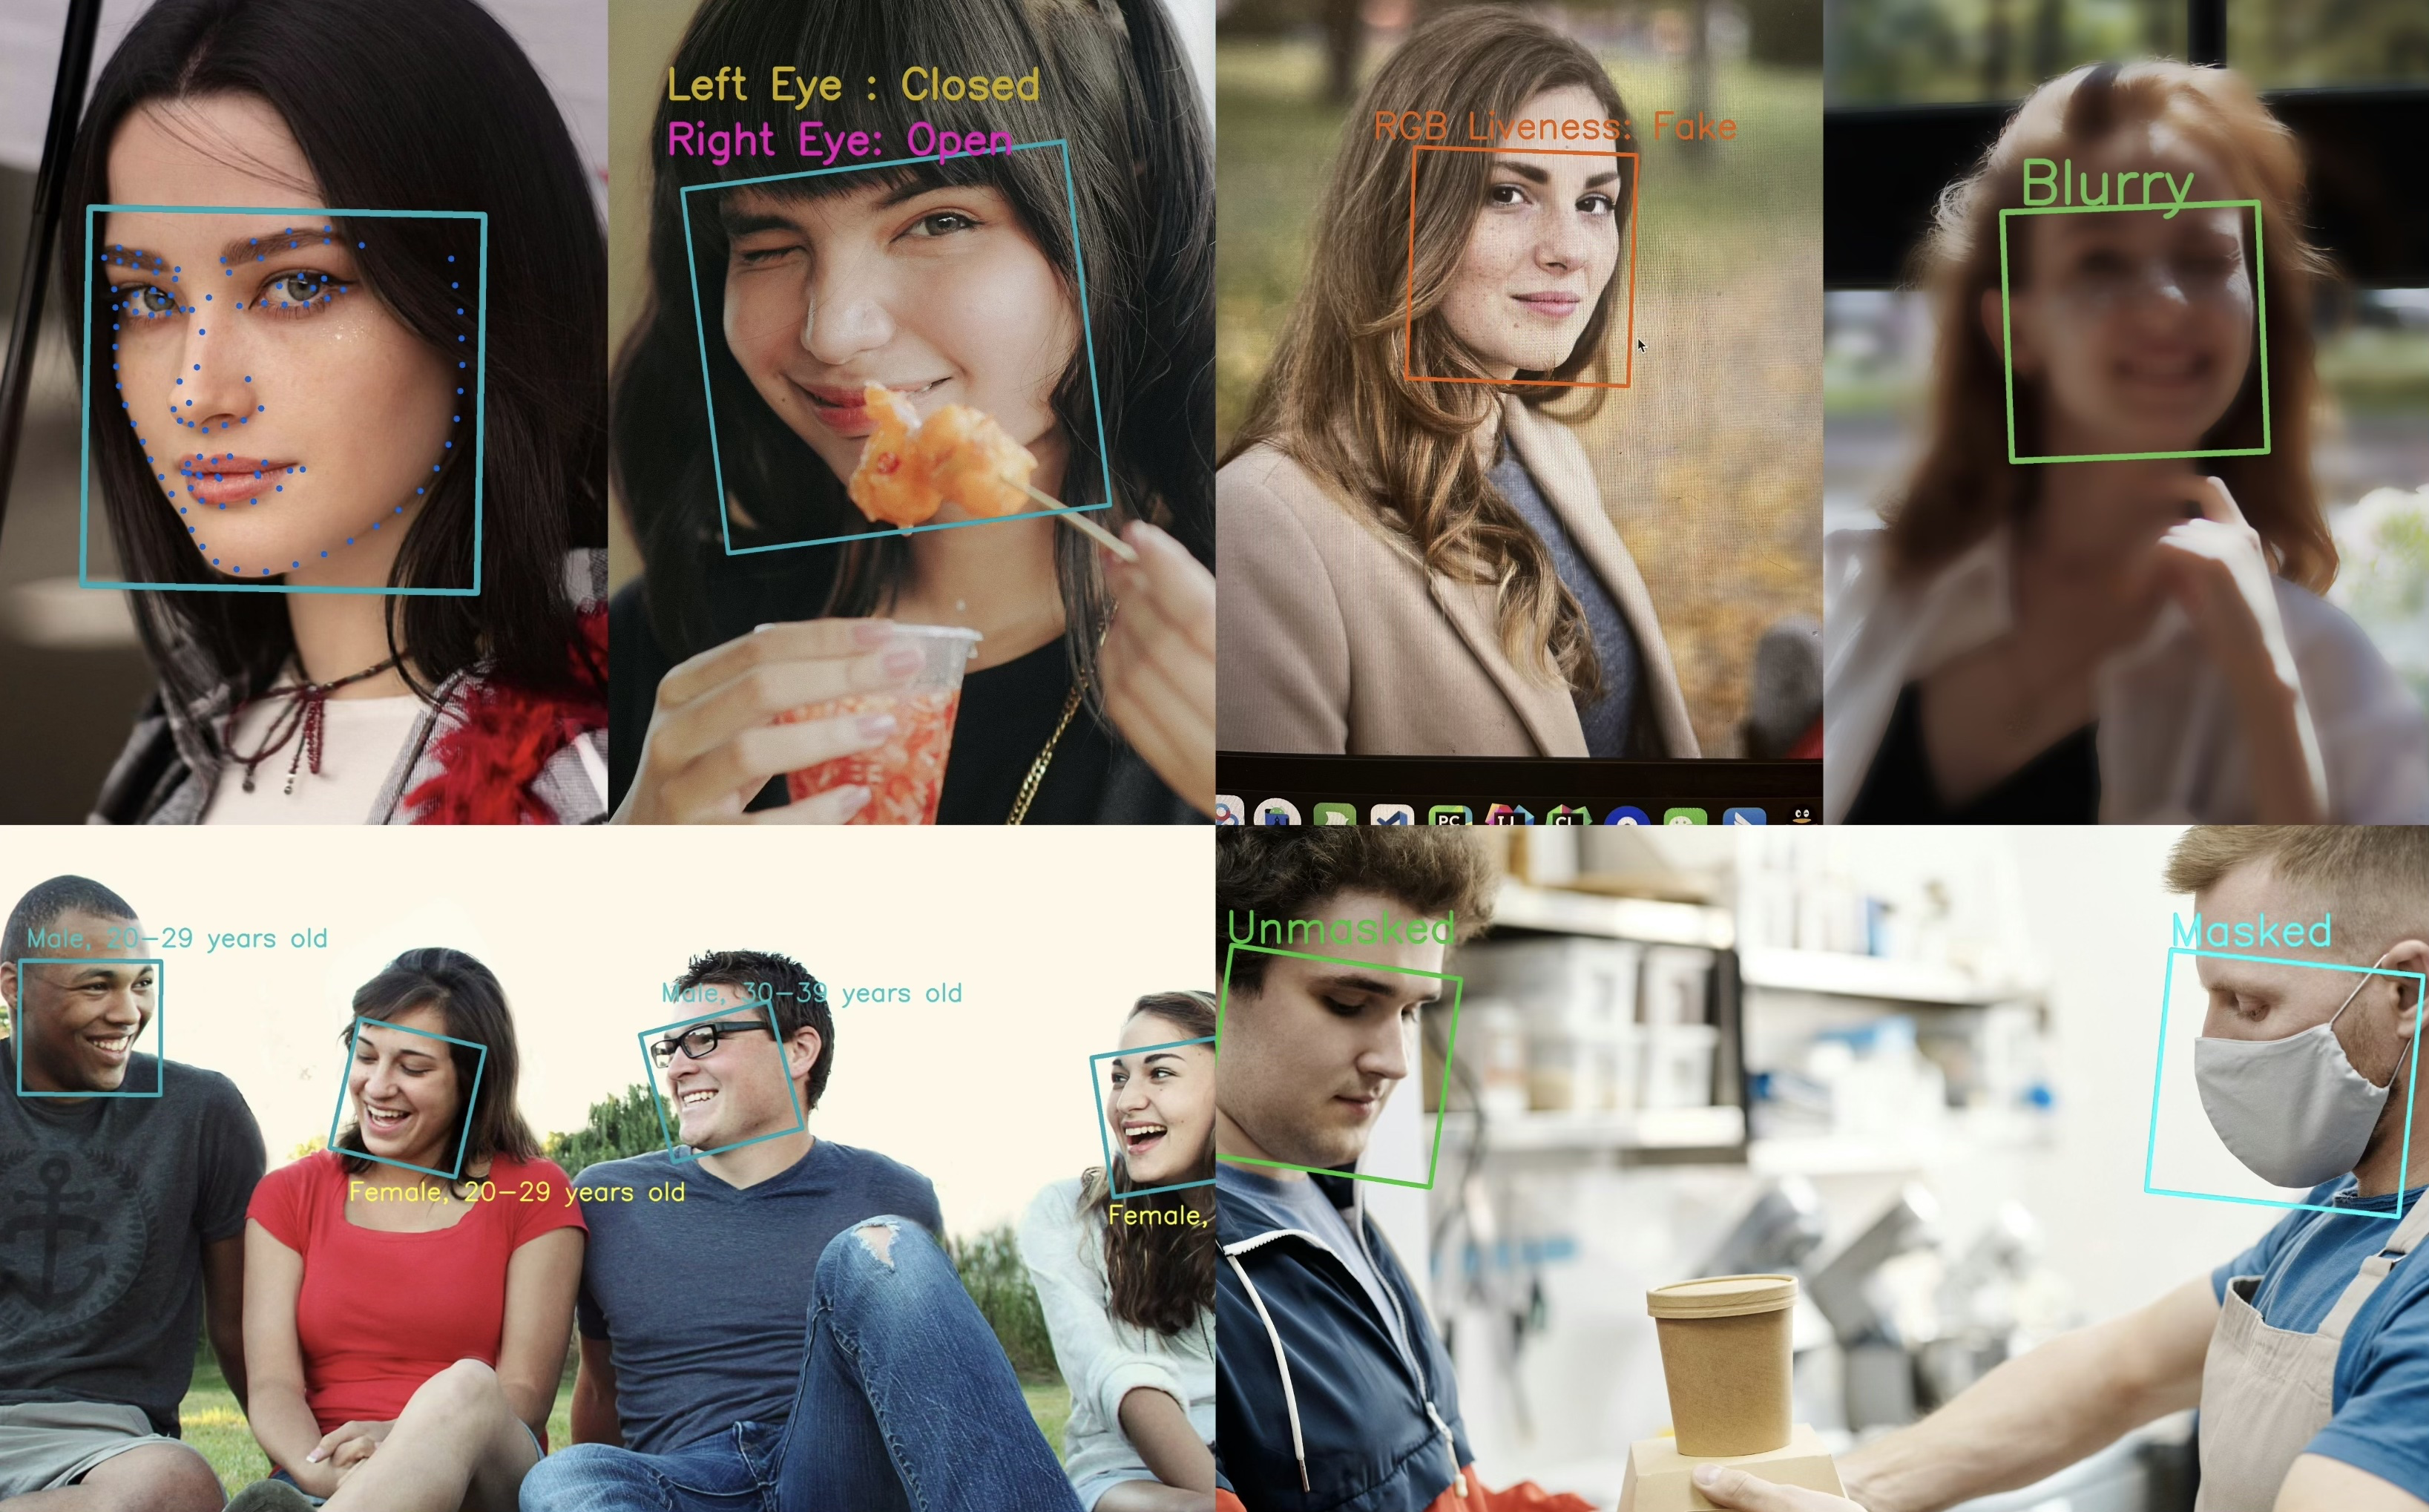
\includegraphics[width=\linewidth]{face_detection/InspireFace.png}
  \end{figure}
  \end{column}
  \end{columns}
\end{frame}

\begin{frame}
  \begin{figure}
    \centering
    \includegraphics[width=0.8\linewidth]{face_detection/inspireface普遍偏低,但区分度差不多.jpg}
    \includegraphics[width=0.8\linewidth]{face_detection/其他模型对比_inspireface.png}
    \caption{InspireFace 相似度低一些,但区分度差不多}
  \end{figure}
\end{frame}

\section{连续性优化}

\begin{frame}{连续性优化}
  主要利用
  \begin{itemize}
    \item 利用人脸作为媒介,ReID 统一多个片段
    \item 利用人的位移在时间和空间上的连续性,针对细小的片段无法用人脸 ReID 进行差值补全
  \end{itemize}
\end{frame}

\begin{frame}{只用人脸}
  \centering
  \includemedia[
  width=0.9\linewidth,
  height=0.7\linewidth,
  activate=pageopen,
  addresource=video/1/face_only.mp4,
  flashvars={source=video/1/face_only.mp4}
  ]{}{VPlayer.swf}
\end{frame}


\section{TODO}

\begin{frame}{TODO}
  单视角人物追踪、利用人脸 ReID 效果基本可行
  \begin{itemize}
    \item 统一多视角
    \item 利用多视角提升球追踪效果
    \item 利用多视角、根据人的位置连续性、不突变特性优化提升人物追踪,人脸检索效果
    \item 二维重建
  \end{itemize}
\end{frame}

\begin{frame}[allowframebreaks]{参考文献}
  \bibliographystyle{thubeamer}
  \bibliography{reference}
\end{frame}

\begin{frame}
  \begin{center}
    {\Huge\calligra Thanks for your attention!}
  \end{center}
\end{frame}

% 结束文档撰写
\end{document}
